\documentclass[a4paper]{article}

\def\ntitle{Quantum Mechanics}
\def\ndate{Michaelmas, 2017 -- 2018}

\ifx \nauthor\undefined
  \def\nauthor{Qiangru Kuang}
\else
\fi

\ifx \ntitle\undefined
  \def\ntitle{Template}
\else
\fi

\ifx \nauthoremail\undefined
  \def\nauthoremail{qk206@cam.ac.uk}
\else
\fi

\ifx \ndate\undefined
  \def\ndate{\today}
\else
\fi

\title{\ntitle}
\author{\nauthor}
\date{\ndate}

%\usepackage{microtype}
\usepackage{mathtools}
\usepackage{amsthm}
\usepackage{stmaryrd}%symbols used so far: \mapsfrom
\usepackage{empheq}
\usepackage{amssymb}
\let\mathbbalt\mathbb
\let\pitchforkold\pitchfork
\usepackage{unicode-math}
\let\mathbb\mathbbalt%reset to original \mathbb
\let\pitchfork\pitchforkold

\usepackage{imakeidx}
\makeindex[intoc]

%to address the problem that Latin modern doesn't have unicode support for setminus
%https://tex.stackexchange.com/a/55205/26707
\AtBeginDocument{\renewcommand*{\setminus}{\mathbin{\backslash}}}
\AtBeginDocument{\renewcommand*{\models}{\vDash}}%for \vDash is same size as \vdash but orginal \models is larger
\AtBeginDocument{\let\Re\relax}
\AtBeginDocument{\let\Im\relax}
\AtBeginDocument{\DeclareMathOperator{\Re}{Re}}
\AtBeginDocument{\DeclareMathOperator{\Im}{Im}}
\AtBeginDocument{\let\div\relax}
\AtBeginDocument{\DeclareMathOperator{\div}{div}}

\usepackage{tikz}
\usetikzlibrary{automata,positioning}
\usepackage{pgfplots}
%some preset styles
\pgfplotsset{compat=1.15}
\pgfplotsset{centre/.append style={axis x line=middle, axis y line=middle, xlabel={$x$}, ylabel={$y$}, axis equal}}
\usepackage{tikz-cd}
\usepackage{graphicx}
\usepackage{newunicodechar}

\usepackage{fancyhdr}

\fancypagestyle{mypagestyle}{
    \fancyhf{}
    \lhead{\emph{\nouppercase{\leftmark}}}
    \rhead{}
    \cfoot{\thepage}
}
\pagestyle{mypagestyle}

\usepackage{titlesec}
\newcommand{\sectionbreak}{\clearpage} % clear page after each section
\usepackage[perpage]{footmisc}
\usepackage{blindtext}

%\reallywidehat
%https://tex.stackexchange.com/a/101136/26707
\usepackage{scalerel,stackengine}
\stackMath
\newcommand\reallywidehat[1]{%
\savestack{\tmpbox}{\stretchto{%
  \scaleto{%
    \scalerel*[\widthof{\ensuremath{#1}}]{\kern-.6pt\bigwedge\kern-.6pt}%
    {\rule[-\textheight/2]{1ex}{\textheight}}%WIDTH-LIMITED BIG WEDGE
  }{\textheight}% 
}{0.5ex}}%
\stackon[1pt]{#1}{\tmpbox}%
}

%\usepackage{braket}
\usepackage{thmtools}%restate theorem
\usepackage{hyperref}

% https://en.wikibooks.org/wiki/LaTeX/Hyperlinks
\hypersetup{
    %bookmarks=true,
    unicode=true,
    pdftitle={\ntitle},
    pdfauthor={\nauthor},
    pdfsubject={Mathematics},
    pdfcreator={\nauthor},
    pdfproducer={\nauthor},
    pdfkeywords={math maths \ntitle},
    colorlinks=true,
    linkcolor={red!50!black},
    citecolor={blue!50!black},
    urlcolor={blue!80!black}
}

\usepackage{cleveref}



% TODO: mdframed often gives bad breaks that cause empty lines. Would like to switch to tcolorbox.
% The current workaround is to set innerbottommargin=0pt.

%\usepackage[theorems]{tcolorbox}





\usepackage[framemethod=tikz]{mdframed}
\mdfdefinestyle{leftbar}{
  %nobreak=true, %dirty hack
  linewidth=1.5pt,
  linecolor=gray,
  hidealllines=true,
  leftline=true,
  leftmargin=0pt,
  innerleftmargin=5pt,
  innerrightmargin=10pt,
  innertopmargin=-5pt,
  % innerbottommargin=5pt, % original
  innerbottommargin=0pt, % temporary hack 
}
%\newmdtheoremenv[style=leftbar]{theorem}{Theorem}[section]
%\newmdtheoremenv[style=leftbar]{proposition}[theorem]{proposition}
%\newmdtheoremenv[style=leftbar]{lemma}[theorem]{Lemma}
%\newmdtheoremenv[style=leftbar]{corollary}[theorem]{corollary}

\newtheorem{theorem}{Theorem}[section]
\newtheorem{proposition}[theorem]{Proposition}
\newtheorem{lemma}[theorem]{Lemma}
\newtheorem{corollary}[theorem]{Corollary}
\newtheorem{axiom}[theorem]{Axiom}
\newtheorem*{axiom*}{Axiom}

\surroundwithmdframed[style=leftbar]{theorem}
\surroundwithmdframed[style=leftbar]{proposition}
\surroundwithmdframed[style=leftbar]{lemma}
\surroundwithmdframed[style=leftbar]{corollary}
\surroundwithmdframed[style=leftbar]{axiom}
\surroundwithmdframed[style=leftbar]{axiom*}

\theoremstyle{definition}

\newtheorem*{definition}{Definition}
\surroundwithmdframed[style=leftbar]{definition}

\newtheorem*{slogan}{Slogan}
\newtheorem*{eg}{Example}
\newtheorem*{ex}{Exercise}
\newtheorem*{remark}{Remark}
\newtheorem*{notation}{Notation}
\newtheorem*{convention}{Convention}
\newtheorem*{assumption}{Assumption}
\newtheorem*{question}{Question}
\newtheorem*{answer}{Answer}
\newtheorem*{note}{Note}
\newtheorem*{application}{Application}

%operator macros

%basic
\DeclareMathOperator{\lcm}{lcm}

%matrix
\DeclareMathOperator{\tr}{tr}
\DeclareMathOperator{\Tr}{Tr}
\DeclareMathOperator{\adj}{adj}

%algebra
\DeclareMathOperator{\Hom}{Hom}
\DeclareMathOperator{\End}{End}
\DeclareMathOperator{\id}{id}
\DeclareMathOperator{\im}{im}
\DeclareMathOperator{\coker}{coker}
\DeclarePairedDelimiter{\generation}{\langle}{\rangle}

%groups
\DeclareMathOperator{\sym}{Sym}
\DeclareMathOperator{\sgn}{sgn}
\DeclareMathOperator{\inn}{Inn}
\DeclareMathOperator{\aut}{Aut}
\DeclareMathOperator{\GL}{GL}
\DeclareMathOperator{\SL}{SL}
\DeclareMathOperator{\PGL}{PGL}
\DeclareMathOperator{\PSL}{PSL}
\DeclareMathOperator{\SU}{SU}
\DeclareMathOperator{\UU}{U}
\DeclareMathOperator{\SO}{SO}
\DeclareMathOperator{\OO}{O}
\DeclareMathOperator{\PSU}{PSU}
\DeclareMathOperator{\Sp}{Sp}


%hyperbolic
\DeclareMathOperator{\sech}{sech}

%field, galois heory
\DeclareMathOperator{\ch}{ch}
\DeclareMathOperator{\gal}{Gal}
\DeclareMathOperator{\emb}{Emb}



%ceiling and floor
%https://tex.stackexchange.com/a/118217/26707
\DeclarePairedDelimiter\ceil{\lceil}{\rceil}
\DeclarePairedDelimiter\floor{\lfloor}{\rfloor}


\DeclarePairedDelimiter{\innerproduct}{\langle}{\rangle}

%\DeclarePairedDelimiterX{\norm}[1]{\lVert}{\rVert}{#1}
\DeclarePairedDelimiter{\norm}{\lVert}{\rVert}



%Dirac notation
%TODO: rewrite for variable number of arguments
\DeclarePairedDelimiterX{\braket}[2]{\langle}{\rangle}{#1 \delimsize\vert #2}
\DeclarePairedDelimiterX{\braketthree}[3]{\langle}{\rangle}{#1 \delimsize\vert #2 \delimsize\vert #3}

\DeclarePairedDelimiter{\bra}{\langle}{\rvert}
\DeclarePairedDelimiter{\ket}{\lvert}{\rangle}




%macros

%general

%divide, not divide
\newcommand*{\divides}{\mid}
\newcommand*{\ndivides}{\nmid}
%vector, i.e. mathbf
%https://tex.stackexchange.com/a/45746/26707
\newcommand*{\V}[1]{{\ensuremath{\symbf{#1}}}}
%closure
\newcommand*{\cl}[1]{\overline{#1}}
%conjugate
\newcommand*{\conj}[1]{\overline{#1}}
%set complement
\newcommand*{\stcomp}[1]{\overline{#1}}
\newcommand*{\compose}{\circ}
\newcommand*{\nto}{\nrightarrow}
\newcommand*{\p}{\partial}
%embed
\newcommand*{\embed}{\hookrightarrow}
%surjection
\newcommand*{\surj}{\twoheadrightarrow}
%power set
\newcommand*{\powerset}{\mathcal{P}}

%matrix
\newcommand*{\matrixring}{\mathcal{M}}

%groups
\newcommand*{\normal}{\trianglelefteq}
%rings
\newcommand*{\ideal}{\trianglelefteq}

%fields
\renewcommand*{\C}{{\mathbb{C}}}
\newcommand*{\R}{{\mathbb{R}}}
\newcommand*{\Q}{{\mathbb{Q}}}
\newcommand*{\Z}{{\mathbb{Z}}}
\newcommand*{\N}{{\mathbb{N}}}
\newcommand*{\F}{{\mathbb{F}}}
%not really but I think this belongs here
\newcommand*{\A}{{\mathbb{A}}}

%asymptotic
\newcommand*{\bigO}{O}
\newcommand*{\smallo}{o}

%probability
\newcommand*{\prob}{\mathbb{P}}
\newcommand*{\E}{\mathbb{E}}

%vector calculus
\newcommand*{\gradient}{\V \nabla}
\newcommand*{\divergence}{\gradient \cdot}
\newcommand*{\curl}{\gradient \cdot}

%logic
\newcommand*{\yields}{\vdash}
\newcommand*{\nyields}{\nvdash}

%differential geometry
\renewcommand*{\H}{\mathbb{H}}
\newcommand*{\transversal}{\pitchfork}
\renewcommand{\d}{\mathrm{d}} % exterior derivative

%number theory
\newcommand*{\legendre}[2]{\genfrac{(}{)}{}{}{#1}{#2}}%Legendre symbol

%algebraic geometry
\DeclareMathOperator{\Spec}{Spec}
\DeclareMathOperator{\Proj}{Proj}

\newtheorem*{postulate}{Postulate}

\begin{document}
\maketitle

\tableofcontents

\setcounter{section}{-1}
\section{Introduction}

Quantum mechaniccs is a radical generalisation of classical physics involving a new fundamental constant, \emph{Planck's constant},
\[
  \hbar = h/2\pi \approx 1.05\times 10^{-34} Js
\]

Profund new features of quantum mechanics include:
\begin{description}
\item[Quantisation] Physical quantities such as energy may be restricted to discrete sets of values, or may appear only in specific amounts, called \emph{quanta}.
\item[Wave-particle duality] Classical concepts of a particle and a wave are merged; they become different aspects of a single eneity that shows either particle-like or wave-like behaviour, depending on the circumstances.
\item[Probability and undertainty]
\end{description}

Despite these radical changes, classical physics must be recovered in the limit $\hbar \to 0$ (which may require careful interpretation).

The followint sections provide some physical background and summarise key experimental evidence for these novel features of quantum mechanics.

\subsection{Light Quanta}

An electromagnetic (EM) wave, e.g. light, consists of quanta called \emph{photons}. Photons can be regarded as particles with energy, $E$, and momentum, $p$, related to frequence, $\nu$ or $\omega$, and wavelength $\lambda$, or wavenumber, $k$, according to
\begin{alignat*}{2}
  E &= h\nu &&= \hbar \omega \\
  p &= h/\lambda &&= \hbar k
\end{alignat*}

From the wave equation (satisfied by each EM field component)
\[
  c= \omega/k = \nu\lambda \: \text{or } E=cp
\]
and so the relations above are consistent with photons being particles of rest mass zero, moving with the speed of light, $c$.

Compelling evidence for the existence of photons is provided by the \emph{photoelectric effect}. Consider light or EM radiation ($\gamma$) of frequence $\omega$ incident on a metal surface. For certain metals and suitable frequencies this results in the emission of electrons ($e^-$) and their maximum kinetic energy $K$ can be measured.

Experiments find that
\begin{enumerate}
\item the rate at which electrons are emitted is proportional to the intensity of the radiation (the `brightness' of the source);
\item $K$ depends linearly on $\omega$ but \emph{not} on the intensity;
  \item for $\omega < \omega_0$, some critical value, \emph{no} electrons are emitted, irrespective of the intensity.
\end{enumerate}

These results are extremely hard to understand in terms of classical EM waves. However, they follow naturally from the assumption that the wave consists of photons, each with energy $E=\hbar\omega$, and with the intensity of the radiation proportional to the number of photons incident per unit time. Suppose that an electron is emitted as a result of absorbing a single photon with sufficiently high energy. If $W$ is the minimum energy needed to liberate an electron from the metal then
\[
  K=\hbar\omega-W
\]
is the maximum kinetic energy of an emitted electron if $\omega>\omega_0$, where $\omega_0=W/\hbar$, and no emission is possible if $\omega<\omega_0$. Furthermore, the rate at which electrons are emitted wil be proportional to the rate at which incident photons arrive, and hence the intensity.

The energy-frequency relation for photons was introduced by Planck and used to derive the \emph{black body spectrum}. This is the distribution of energy with frequency for EM radiation in thermal euqilibrium, a fundamental result in thermodynamics of far-reaching importance (understanding the \emph{cosmic microwave background}, for example). Einstein then applied the energy-frequency relation to explain the photoelectric effect. Further conclusive evidence for photons as particles, including the momentum-wavelength relation, came from subsequent experiments involving \emph{Compton scattering}.

Consider a photon of wavelength $\lambda$ colliding with an electron that is statioinary in the laboratory frame. Let $\lambda'$ be the wavelength of the photon after the collision and $\theta$ the angle through which it is deflected. Treating the photon as a massless relativistic particle, conservation of four-momentum imples
\[
  \lambda'-\lambda = \frac{h}{m_e c}(1-\cos \theta).
\]
This dependence of the change in wavelength (or decrease in energy) on the scattering angle $\theta$ can be verified experimentally (for X-rays or $\gamma$-rays, for instance).

\subsection{The Bohr Model of the Atom}

The \emph{Rutherford model} of the atom was proposed to explain the results of scattering experiments (e.g. alpha particles scattered by gold foil). The key assumption is that most of the mass of the atom is concentrated in a compact, positively-charged \emph{nucleus} (subsequently understood to consist of protons and neutrons), with light, negatively-charged electrons orbiting aroundit. The simplest case is the hydrogen atom, in which a single electron with charge $-e$ and mass $m_e$ orbits a nucleus consisting of a single proton with charge $+e$ and mass $m_p$. Since $m_p >> m_e$ it is a good approximation to assume that the proton is stationary, at the origin, say. The electron and proton interact via Coulomb's Law: the potential energy of the electron and the force it experiences are
\[
  V(r) = -\frac{e^2}{4\pi \epsilon_0} \frac{1}{r},\: \V F(\V r) = -\nabla V = -\frac{e^2}{4\pi \epsilon_0}\frac{1}{r^2} \hat{\V r}.
\]

The classical equations of motion for the electron imply that its angular momentum, $\V L = \V r \times \V p$, and its total energy,
\[
  E=\frac{1}{2}m_e v^2 - \frac{e^2}{4\pi\epsilon_0}\frac{1}{r},
\]
are constant. The orbits are therefore planar and they can be determined exactly. For any value of $E<0$ there is a closed orbit and the electron is \emph{bound} to the proton to form a hydrogen atom. For orbits with $E>0$ the electron eventually escapes to infinity: it is not bound to the proton.

Despite the success in accounting for Rutherford scattering, this model has a number of problems. The treatment is identical, mathematically, to planetary orbits governed by gravity but an importatnt additional feature of electromagnetism has been left out. An accelerating charge radiates energy and this means that the electron will actually spiral inwards towards the proton: this is not a good model of a stable atom.

There is also experimental evidence for complex discrete structure within atoms. This comes from \emph{line spectra}: brigh emission lines (from a hot sample) or dark absorption lines (if radiation is passed through a cooler sample), both occuring at certain characteristic wavelengths or frequencies. This suggests that an atom can emit or absorb radiation only at there particular frequencies or wavelengths, which correspond to photons with particular energies.

The \emph{Bohr model} restricts the classical orbits of the Rutherford model by postulating that the angular momentum of the electron obeys the \emph{Bohr quantisation condition}:
\[
  L = n\hbar, n=1,2,\ldots,
\]
with only these discrete values allowed. This might seem to be an unsatisfactory way to address the issue of stability, but it proves to be remarkably successful in reproducing the complex experimental data relating to line spectra.

Specialising to circular orbits, for simplicity, we have
\[
  F=m_e v^2/r, L=m_e rv.
\]
It is then straightforward to check that the quantisation condition leads to the following set of \emph{Bohr orbits}:
\begin{align*}
  r_n &= \frac{4\pi\epsilon_0\hbar^2}{m_e e^2}n^2 \\
  v_n &= \frac{e^2}{4\pi\epsilon_0\hbar}\frac{1}{n} \\
  E_n &= -\frac{1}{2}m_e (\frac{e^2}{4\pi\epsilon_0\hbar})^2\frac{1}{n^2},\: n =1,2,\ldots
\end{align*}
Note that the allowed energy levels are now discrete.

Suppose that an electron makes a transition between levels $n$ and $n'$ (with $n' > n$, say) accompanied by emission or absorption of a photon of frequency $\omega$. Then
\[
  \hbar\omega = E_{n'} - E_n = \frac{1}{2}m(\frac{e^2}{4\pi\epsilon_0\hbar})^2 (\frac{1}{n^2} - \frac{1}{n'^2}).
\]

This formula accounts for a vast amount of experimental data on spectral lines for hydrogen. The Bohr model also provides an estimate for the \emph{size} of the hydrogen atom $r_1 \approx 5.29\times 10^{-11} m$, the \emph{Bohr radius}. Despite these considerable successes, the origin of the Bohr quantisation condition seems obscure. A better explanation is needed.

\subsection{Matter Waves}

The relations used to associate particle properties ($E$ and $p$) to waves can also be used to associate wave properties ($\nu$ or $\omega$ and $\lambda$ and $k$) to particles. This applies not just to relativistic photons but also to non-relativisitic particles, electrons for example, and $\lambda$ is called the \emph{de Broglie wavelength} of the particle. A strong hint that this might be important for a better understanding of the Bohr quantisatoin condition comes from observing that for a circular orbit
\[
  L = rp = n\hbar \Leftrightarrow n\lambda = 2\pi r.
\]
The Bohr condition therefore says that the circumference of the orbit is exactly an integral number of de Broglie wavelengths (e.g. $n=3$ in the figure).

It can also be verified experimentally that electrons do indeed exhibit wave-like behaviour, and a helpful idealisaton is the \emph{double slit experiment}. Consider a source which emits a beam of electrons, a barrier with two slits that can be open or closed, and a screen on which the electrons are detected.

Suppose first that one slit is open and the other is closed, as in Figure. We cannot say with certainty where any particular electron will be detected, but after many electrons have been emitted, the number detected varies with transverse position according to the distributions shown. If \emph{both} slits are open, however, then the electrons produce (perhaps unexpectedly) an interference pattern (Fig).

This matches the interference pattern obtained for waves of wavelength $\lambda$ incident on a barrier, as shown in Fig. Consider a point $P$ at some fixed perpendicular distance from the barrier, and let $\delta$ be the difference of the distances to $P$ from each of the slits. Constructive interference occurs for $\delta=n\lambda$ while destructive interference occurs for $\delta=(n+1/2)\lambda$. The result is that the suare of the amplitude of the superposed waves varies as shown in Fig, as $P$ varies.

In diffraction expreiments with electrons, we cannot predict what will happen to any \emph{single} particle; the most that can be said is that it will be detected at a given position with a certain \emph{probability}. The diffraction pattern is conclusive evidence of interference and so confirms the existence of matter waves, and diffraction expreiments allow an experimental determination of the de Broglie wavelength. The results also suggest that the probability distribution for particles can be expressed as the square of the amplitude of a wave.

\section{Wavefunctions and Operators}

In the first few sections we consider quantum particle in one dimension and introduce some key ideas and three postulates for how to extract physical information from mathematical framework. Later we will state general axioms from which these follow.

\subsection{Wavefunctions and States}

A classical point particle in one dimensional has a position $x$ at each time. In quantum mechanis a particle has a \emph{state} at each time given by a complex-valued wavefunction $\psi(x)$.

\begin{postulate}[P1]
  \label{postulate:1}
  A measurement of position gives a result with probability density $|\psi(x)|^2$. In other words, $|\psi(x)|^2 \delta x$ is the probability that the particle is found between $x$ and $x+\delta x$. Equivalently, $\int_a^b |\psi(x)|^2 dx$ is the probability that the particle is found in $[a,b]$.
\end{postulate}

This requires that $\psi(x)$ is \emph{normalised}:
\[
  \int_{-\infty}^\infty |\psi(x)|^2 dx = 1.
\]

\begin{eg}[Gaussian wavefunction]
  Let $\psi(x) = C e^{-(x-x_0)^2/2\alpha}$ for some real $\alpha>0$.
  \begin{center}
  \begin{tikzpicture}
    \begin{axis}[
      ticks=none,
      axis equal image,
      axis lines=center,
      xmin=-1,
      xmax=7,
      ymin=-0.2,
      ymax=2,
      xlabel=$x$,
      ylabel=$|\psi(x)|^2$]
     \addplot[restrict x to domain=-1:7,color=red,samples=80]{exp{-(x-3)^2}};
    \end{axis}
  \end{tikzpicture}
  \end{center}
  \begin{align*}
    \int_{-\infty}^\infty |\psi(x)|^2 dx &= |C|^2 \int_{-\infty}^\infty e^{-(x-x_0)^2/\alpha} dx \\
    &= |C|^2 (\alpha\pi)^{1/2} \\
    &= 1
  \end{align*}
  So $\psi$ is normalised if $C=(\frac{1}{\alpha\pi})^{1/4}$. If $\alpha$ is small, there is a sharp peak around $x=x_0$, and it exhibits ``particle-like'' behaviour. If $\alpha$ is large, it is more spread out/diffused.
\end{eg}

It is convenient to deal more generaly with \emph{normalisable} wavefunctions satisfying
\[
  \int_{-\infty}^\infty |\psi(x)|^2 dx < \infty,
\]
i.e. the integral is finite/convergent. Then $\psi(x)$ and $\phi(x) = \lambda\psi(x)$ are physically equivalent and represent the same state for any $\lambda\neq0$. Provided $\psi$ is normalisable, we can choose $\lambda$ so that $\phi$ is normalised. But if $\psi$ is normalised already, $\phi(x) = e^{i\alpha}\psi(x)$ for any real $\alpha$ gives the same probability distribution $|\phi(x)|^2 = |\psi(x)|^2$. This means that quantum state is strictly an equivalence class of non-zero wavefunctions but in practice we often refer to $\psi(x)$ as ``the state''.

Any non-zero normalisable wavefunction $\psi(x)$ represents a physical state. For our purpose we can assume, unless we say otherwise,
\begin{assumption}\leavevmode
\begin{itemize}
\item $\psi(x)$ is smooth, i.e. can be differeniated any number of times, and
  \item $\psi(x) \to 0$ as $|x|\to\infty$.
\end{itemize}
\end{assumption}

If $\psi_1(x)$ and $\psi_2(x)$ are normalisble then so is
\[
  \psi = \lambda_1\psi_1 + \lambda_2\psi_2
\]
for any complex numbers $\lambda_1, \lambda_2$. Physically, this is the principle of superposition and mathematically, this endows the space of normalisable wavefunctions a complex vector space structure.

\begin{eg}[Superposition of Gaussians]
  Let $\psi(x) = B(e^{-x^2/2\alpha}+e^{-(x-x_0)^2/2\alpha})$. We can choose $B$ so that $\psi$ is normalised.
  \begin{center}
  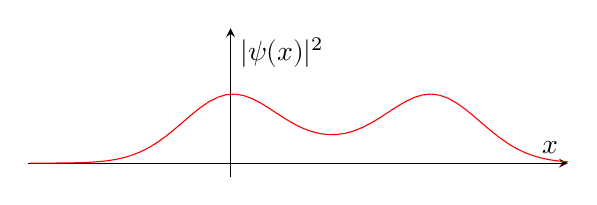
\begin{tikzpicture}
    \begin{axis}[
      ticks=none,
      axis equal image,
      axis lines=middle,
      xmin=-3,
      xmax=5,
      ymin=-.2,
      ymax=2,
      xlabel=$x$,
      ylabel=$|\psi(x)|^2$]
     \addplot[restrict x to domain=-3:5, color=red,samples=80]{(exp{-x^2}/2+exp{-(x-3)^2}/2)^2};
    \end{axis}
  \end{tikzpicture}
  \end{center}
 
\end{eg}

\subsection{Operators and Observables}

A quantum state contains information about other physical quantities or \emph{observables}, such as momentum and energy, not just position. In quantum mechanics, each observable is represented by an \emph{operator} (denoted by a hat when necessary) acting on wavefunctions. For example:
\begin{itemize}
  \item position: $\hat x = x, (\hat{x}\psi)(x) = x\psi(x)$,
  \item momentum: $\hat{p} = -i\hbar \frac{d}{dx}, (\hat{p}\psi)(x) = -i\hbar\psi'(x)$,
  \item energy/Hamiltonian: $H = \frac{1}{2m}\hat{p} + V(\hat{x}) = -\frac{\hbar^2}{2m}\frac{d^2}{dx^2} + V(x)$ for a particle of mass $m$ in a potential $V$.
  \end{itemize}

If we measure one of these quantities, what answers can we get and what are the probabilities? Partial answers are provides by P2 and P3.

\subsubsection{Expectation Value}

For any (normalisable) $\psi(x)$ and $\phi(x)$, define
\[
  (\psi, \phi) = \int_{-\infty}^\infty \psi(x)^* \phi(x) dx,
\]
the complex inner product on the vector space. For $\psi(x)$ normalised, define the \emph{expectation value} of an observable $Q$ in this state to be
\[
  \langle Q \rangle_\psi = (\psi, Q\psi) = \int_{-\infty}^\infty \psi^* Q\psi dx.
\]

Note
\[
  \langle \hat x \rangle_\psi = (\psi, \hat x \psi) = \int_{-\infty}^\infty x |\psi(x)|^2 dx,
\]
the standard expression for mean, or expected value of $x$, given by P1.

\begin{postulate}[P2]
  \label{postulate:2}
  For any observable, $\langle Q\rangle_\psi$ is the mean result (expected value) if $Q$ is measured many times (as times $N\to\infty$) with particle in state $\psi$ before each measurement.
\end{postulate}

Consider wavefunction
\[
  \phi(x) = \psi(x)e^{ikx}
\]
with $k$ a real constant. Clearly
\[
  |\phi(x)|^2 = |\psi(x)|^2
\]
so
\[
  \langle \hat x\rangle_\phi = \langle \hat x\rangle_\psi.
\]
But
\begin{align*}
  \langle\hat p\rangle_\phi &= \int_{-\infty}^\infty \phi^*(-i\hbar\phi')dx \\
  &= \int_{-\infty}^\infty \psi^*(-i\hbar\psi')dx + \hbar k\int_{-\infty}^\infty \psi^*\psi dx \\
  &= \langle \hat p\rangle_\psi + \hbar k
\end{align*}

\begin{eg}
  Let $\psi(x) = Ce^{-x^2/2\alpha}$, then $\langle\hat p\rangle_\psi = 0$ and $\psi(x) = Ce^{-x^2/2\alpha}e^{ikx}$ with $\langle\hat p\rangle_\phi = \hbar k$.
\end{eg}
\end{document}